\section{Introducción}
\label{sec:introduccion}

\subsection{Motivación del trabajo}

La movilidad urbana eficiente constituye uno de los principales desafíos para las ciudades contemporáneas, especialmente en un contexto de creciente demanda de sostenibilidad, aumento del parque automovilístico y limitaciones estructurales de las infraestructuras viarias existentes. Una gestión adecuada del tráfico no solo repercute positivamente en la calidad de vida de la ciudadanía, sino que también tiene un impacto directo en la reducción del consumo energético, la mejora de la seguridad vial y la disminución de la contaminación atmosférica.

En este escenario, la predicción del tráfico emerge como una herramienta clave para anticiparse a situaciones de congestión, disrupciones u otros eventos que puedan comprometer la fluidez de la circulación. La inteligencia Artificial y, en particular, del Aprendizaje Profundo, ha impulsado el desarrollo de modelos que integran datos en tiempo real y capturan patrones complejos mediante el uso de arquitecturas sofisticadas.

El creciente interés por aplicar estos avances en entornos reales de alta densidad urbana motiva la realización del presente trabajo, que se centra en el desarrollo de un modelo de predicción de tráfico con enfoque local en la provincia de Bizkaia, uno de los territorios más dinámicos y problemáticos desde el punto de vista de la movilidad en el norte de España.

\subsection{Planteamiento del problema}

La provincia de Bizkaia presenta un conjunto de particularidades que complican la gestión efectiva del tráfico. Su orografía abrupta limita la expansión de nuevas vías y condiciona la distribución del tráfico en corredores específicos, donde la saturación es frecuente. A esto se suma la alta densidad poblacional, especialmente en el área metropolitana de Bilbao, y una variabilidad meteorológica significativa, que puede afectar las condiciones de circulación de forma impredecible.

\begin{figure}[H]
	\centering
	\caption[Red viaria de la CAPV]{Red viaria de la CAPV}
	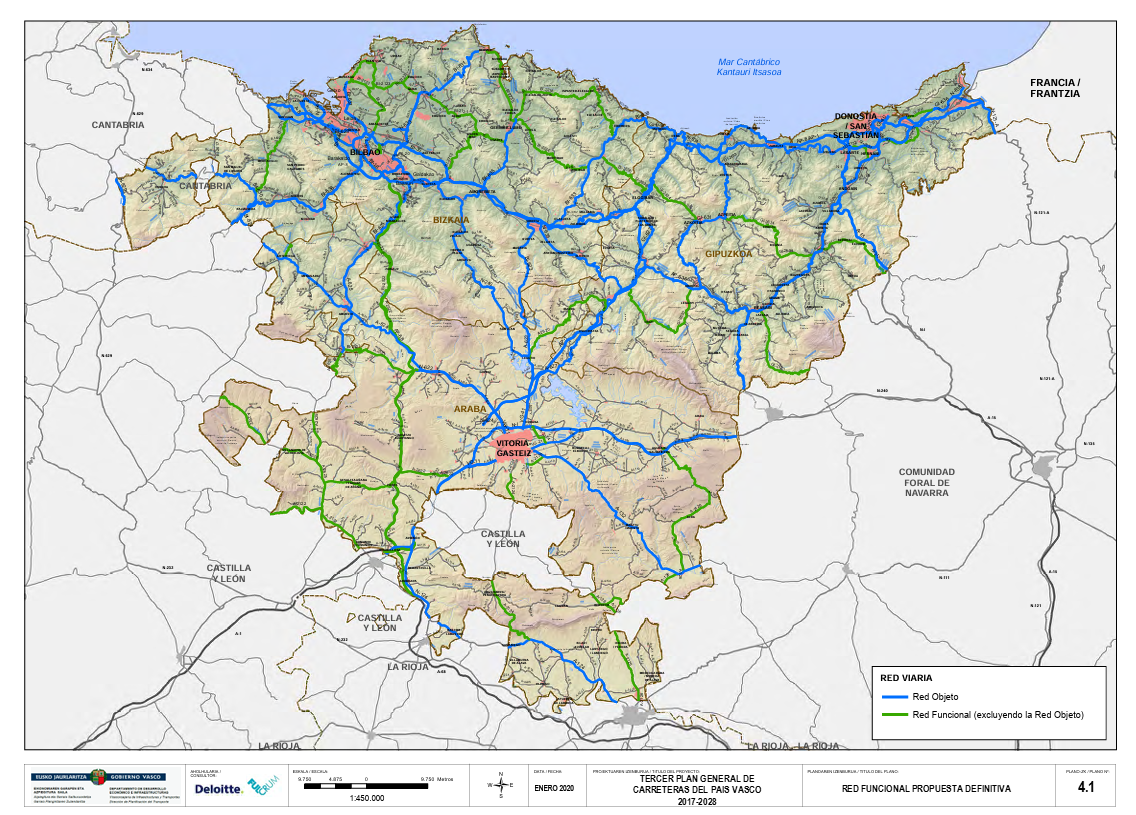
\includegraphics[scale=0.5]{includes/red_viaria_capv.png}
	\label{fig:red_viaria}
\end{figure}
\fuente{\cite{pgcpv}. \textit{Tercer Plan General de Carreteras del País Vasco 2017-2028.}}

En la figura \ref{fig:red_viaria} se aprecia la complejidad de la red viaria en la \acrshort{capv}. En diversas zonas como los accesos a Bilbao, los túneles del Kadagua o los enlaces con la A-8, se producen episodios de congestión recurrentes, especialmente en horas punta y durante condiciones meteorológicas adversas. Aunque Bizkaia dispone de una infraestructura \acrshort{its} notable (sensores, cámaras, estaciones meteorológicas), no se cuenta aún con herramientas predictivas suficientemente precisas que permitan anticipar estos episodios y facilitar la toma de decisiones en tiempo real.

La complejidad inherente a los datos de tráfico, caracterizados por correlaciones espacio-temporales, no linealidades y gran volumen, exige modelos capaces de capturar dichas relaciones con eficacia. Las aproximaciones tradicionales, basadas en regresión o aprendizaje automático clásico, resultan insuficientes en este contexto. Se necesita un enfoque moderno, capaz de integrar múltiples fuentes de datos y aprender representaciones complejas.

En respuesta a los retos mencionados, este trabajo propone el diseño, desarrollo y evaluación de un modelo de predicción del tráfico en Bizkaia basado en redes neuronales con arquitectura transformer. La elección de este enfoque se fundamenta en los resultados recientes de la literatura, donde modelos como Trafficformer han demostrado una notable capacidad para capturar dependencias espaciotemporales complejas en datos de tráfico y obtener mejores resultados que otras arquitecturas profundas tradicionales, gracias al mecanismo de atención y la integración de información topológica de la red viaria \cite{trafficformer}. Esta evidencia convierte a los Transformers en una opción idónea para abordar la predicción de tráfico con alta precisión en entornos urbanos complejos.

El modelo se alimentará de datos abiertos sobre tráfico y meteorología, publicados por organismos como Open Data Euskadi y Euskalmet, lo que garantiza la transparencia, replicabilidad y aplicabilidad del sistema propuesto. A través de un enfoque empírico, se evaluará la eficacia del modelo frente a enfoques tradicionales, utilizando métricas estándar y se estudiará su potencial para integrarse en sistemas actuales de gestión del tráfico.

Este documento se estructura de la siguiente manera: el capítulo 2 presenta una revisión del estado del arte, analizando los principales trabajos relacionados y su aplicabilidad al contexto de Bizkaia; el capítulo 3 define los objetivos del trabajo y la metodología seguida; el capítulo 4 muestra la construcción del dataset y presenta la arquitectura; el capítulo 5 describe el software desarrollado; en el capítulo 6 se muestra la evaluación y discuten los resultados obtenidos; acabando con el capítulo 7 donde se detallan las conclusiones y el trabajo futuro.
